\documentclass[a4paper]{article}
\usepackage[utf8]{inputenc}
\usepackage[czech]{babel}
\usepackage[T1]{fontenc}

\usepackage[pdftex]{graphicx}
\usepackage{ifpdf}
\usepackage{hyperref}

\title{Scrabble -- Programátorská dokumentace}

\author{Ondrej Profant}

\date{\today}

\ifpdf
\hypersetup{
	pdfauthor={Ondrej Profant},
	pdftitle={Scrabble -- Programátorská dokumentace},
	pdfsubject={Podrobná dokumentace k programu Scrabble: http://github.com/Kedrigern/scrabble},
	pdfkeywords={scrabble, gaddag, trie, mono, monodevelop, csharp, gtk-sharp}
}
\fi

\begin{document}

\tableofcontents	

\section{Použité nástroje}
Program je psán v jazyce C\# (verze 4) a využívá knihoven GTK\#. 
Pro vývoj bylo použito vývojové prostředí MonoDevelop (2.6) a distribuoaný systém správy verzí GIT (1.7.5.4).
Pro tvorbu grafiky Inkscape (0.48), externí dokumentace je psaná v LaTeXu (TeXLive 2009-13). Vyvíjeno na Ubuntu 11.04--11.10.

\section{Zdrojové kódy -- obecně}
\subsection{Získání}
Příkazem:

\texttt{git clone git://github.com/Kedrigern/scrabble.git} 

\noindent
získáte celý projekt. Můžeme ho rozdělit do tří částí:
\begin{enumerate}
\item Scrabble: obsahuje samotný kód v C\#. Soubory v této složce uvidíte i z Monodevelop, více viz kap. \ref{scrabble}.
\item scripts: Obsahuje pomocné skripty, více viz. podkapitola \ref{scripts}.
\item DOC-CS: Obsahuje dokumentaci (včetně \LaTeX{} zdrojových kódů)
\end{enumerate}

\subsection{Využití IDE}
Soubor s koncovkou \texttt{sln} lze otevřít v MonoDevelop, které vám zobrazí celou strukturu zdrojových kódů velmi přehledně, vypadá přibližně takto:

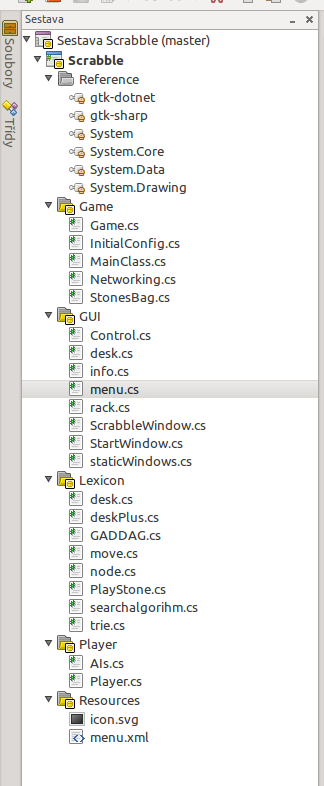
\includegraphics[scale=0.5]{pic/monodevelop-project.png}

Struktura rozdělení zdrojových kódů snad mluví sama za sebe. Většina důležitých tříd a funkcí je komentovaná přímo v kódu -- velká část této dokumentace také vychází rovnou z automaticky vyexportované inline dokumentace. 

Pokud by vám MonoDevelop nevyhovalo, tak můžeme bez problémů použít jinou strukturu (např. MS Visual Studio 2010 používá stejnou).

\subsection{Pomocné skripty}\label{scripts}
V adresáři \texttt{scripts} je serie shellových skriptů, které pomáhají při kompilaci (např. různé druhy kompilace), balíčkování, získávání slovníků etc. 

\section{Zdrojové kódy -- Scrabble}\label{scrabble}
\subsection{Obecně}
\subsection{GADDAG}
\subsection{Podrobná dokumentace tříd}
Zde bych si dovolil odkázat na automaticky generovanou dokumentaci. Ve složce \texttt{scripts} najdete \texttt{makeDoc.sh}, který vám poskytne nejnovější verzi (vygenerována je do složky: \texttt{DOC-CS/htmldoc/}). 

\section{Odkazy}
\begin{description}
\item[git]: \href{http://git-scm.com}{http://git-scm.com}
\item[GitHub]: \href{http://github.com}{http://github.com}
\item[GTK\#]: \href{http://www.mono-project.com/GtkSharp}{http://www.mono-project.com/GtkSharp}
\item[Inkscape]: \href{http://inkscape.org}{http://inkscape.org}
\item[Mono]: \href{http://www.mono-project.com}{http://www.mono-project.com}
\item[MonoDevelop]: \href{http://monodevelop.com}{http://monodevelop.com}
\end{description}

\end{document}
